%==============================================================================
% PAPER 2, CHAPTER 2: Exceptional Lie Algebras and Root Systems
%==============================================================================

\chapter{Exceptional Lie Algebras: The Hidden Symmetries of Nature}
\label{ch:p2:exceptional-lie-groups}

\marginphysics{Exceptional groups unify forces beyond the Standard Model}

\section{Why Exceptional Symmetries Matter}

The Standard Model of particle physics is spectacularly successful, predicting the Higgs boson (discovered 2012), the W and Z bosons (1983), and countless phenomena with stunning precision.\marginhistory{Standard Model: SU(3)$_C \times$ SU(2)$_L \times$ U(1)$_Y$} Yet it has 19 free parameters that must be measured experimentally. Why these particle masses? Why three generations? Why this gauge group?

Grand Unified Theories (GUTs) attempt to answer these questions by embedding the Standard Model into a larger structure.\marginphysics{GUT scale: $\sim 10^{16}$ GeV} The simplest candidate is SU(5) (Georgi-Glashow, 1974), but it predicts proton decay faster than experimental limits allow.

Enter the \textbf{exceptional Lie groups}: $G_2$, $F_4$, $E_6$, $E_7$, and $E_8$. These exotic structures---called ``exceptional'' because they don't fit infinite families---solve many GUT problems:\marginmath{Five exceptional groups, no more}
\begin{itemize}
  \item \textbf{$E_6$}: Contains Standard Model + right-handed neutrinos
  \item \textbf{$E_7$}: Accommodates supersymmetry breaking patterns
  \item \textbf{$E_8$}: Maximal unification in string theory
\end{itemize}

The 2010 CoNb$_2$O$_6$ quantum magnet experiment demonstrated that $E_8$ symmetry emerges in real physical systems at quantum criticality.\marginhistory{Coldea experiment (2010): First $E_8$ observation} This chapter explores the mathematics of exceptional groups and their role in fundamental physics.

\section{From Octonions to Exceptional Groups}
\label{sec:p2:exceptional:motivation}

\subsection{The Non-Associativity Puzzle}

Recall from Chapter~\ref{ch:p2:cayley-dickson} that octonions $\mathbb{O}$ (8D) are non-associative:\marginmath{$(xy)z \neq x(yz)$ for octonions}
\begin{equation}
  (xy)z \neq x(yz)
  \label{eq:p2:exceptional:nonassoc}
\end{equation}

How can we do physics when multiplication doesn't associate? The answer lies in \textbf{automorphisms}---transformations preserving octonionic structure.

\subsection{Automorphism Groups}

An automorphism of the octonions is a linear transformation $g: \mathbb{O} \to \mathbb{O}$ preserving multiplication:\marginmath{Automorphism: $g(xy) = g(x)g(y)$}
\begin{equation}
  g(xy) = g(x) \, g(y) \quad \text{for all } x, y \in \mathbb{O}
  \label{eq:p2:exceptional:automorphism}
\end{equation}

These transformations form a Lie group called $G_2$ (dimension 14). It acts on the 7D space of purely imaginary octonions.\marginphysics{$G_2$ holonomy in M-theory}

\textbf{Physical meaning}: $G_2$ holonomy manifolds appear in M-theory compactifications, preserving $\mathcal{N}=1$ supersymmetry in 4D.

\subsection{The Exceptional Hierarchy}

If $G_2$ preserves octonion multiplication, what preserves $3 \times 3$ Hermitian octonionic matrices?\marginmath{Jordan algebra: $J_3(\mathbb{O})$}

A Hermitian octonionic matrix:
\begin{equation}
  X = \begin{pmatrix}
    \xi_1 & a_3 & \overline{a_2} \\
    \overline{a_3} & \xi_2 & a_1 \\
    a_2 & \overline{a_1} & \xi_3
  \end{pmatrix}, \quad \xi_i \in \mathbb{R}, \, a_i \in \mathbb{O}
  \label{eq:p2:exceptional:albert}
\end{equation}

These form the \textbf{exceptional Jordan algebra} $J_3(\mathbb{O})$. Its automorphism group is $F_4$ (dimension 52).\marginphysics{$F_4$ describes three-qutrit entanglement}

Continuing this pattern yields the full hierarchy:\marginmath{$E_8 \supset E_7 \supset E_6 \supset F_4 \supset G_2$}
\begin{equation}
  E_8 \supset E_7 \supset E_6 \supset F_4 \supset G_2
  \label{eq:p2:exceptional:hierarchy}
\end{equation}

\section{$G_2$: The Smallest Exceptional Group}
\label{sec:p2:exceptional:g2}

\subsection{Definition and Structure}

$G_2$ is the automorphism group of octonions:\marginmath{Dimension: 14}
\begin{equation}
  G_2 = \text{Aut}(\mathbb{O}) = \{ g \in \text{GL}(7,\mathbb{R}) \mid g(xy) = g(x)g(y) \}
  \label{eq:p2:g2:definition}
\end{equation}

\textbf{Root system}: 12 roots in hexagonal pattern with two lengths (ratio $1:\sqrt{3}$)\marginmath{12 roots: 6 short + 6 long}

\textbf{Dynkin diagram}: $\circ \Longleftarrow \circ$ (triple bond indicates different root lengths)\margindim{Triple bond: root ratio $1:\sqrt{3}$}

\subsection{Physical Applications}

\textbf{M-theory compactifications}: Compactifying on a 7D manifold with $G_2$ holonomy preserves $\mathcal{N}=1$ SUSY.\marginphysics{7D compactification: $11 - 4 = 7$}

\textbf{Quark confinement}: Octonion non-associativity (preserved by $G_2$) may explain color confinement in QCD.\margincaution{Speculative but intriguing}

\textbf{Experimental signature}: $G_2$ manifolds predict specific superpartner mass patterns.\marginex{LHC searches: gluino $> 1-2$ TeV}

\section{$F_4$: The Exceptional Jordan Algebra}
\label{sec:p2:exceptional:f4}

\subsection{Definition and Structure}

$F_4$ is the automorphism group of the Albert algebra $J_3(\mathbb{O})$ with Jordan product:\marginmath{Jordan product: commutative}
\begin{equation}
  X \circ Y = \frac{1}{2}(XY + YX)
  \label{eq:p2:f4:jordan-product}
\end{equation}

\textbf{Dimension}: 52\marginmath{52 = 48 roots + 4 Cartan}

\textbf{Root system}: 48 roots (24 short + 24 long, ratio $1:\sqrt{2}$)

\textbf{Dynkin diagram}: $\circ - \circ \Longrightarrow \circ - \circ$

\subsection{Quantum Information Connection}

The 27-dimensional fundamental representation describes the \textbf{entanglement polytope of three qutrits}.\marginphysics{Qutrit: 3-state quantum system}

For three quantum particles with three states each, entanglement patterns form a geometric shape in 27D. The symmetries are precisely $F_4$.\margincomp{Trapped ions, photonic qubits}

The entanglement manifold:\marginmath{$F_4$/Spin(9) coset space}
\begin{equation}
  \mathcal{M}_{\text{entanglement}} = \frac{F_4}{\text{Spin}(9)}
  \label{eq:p2:f4:entanglement-manifold}
\end{equation}

\textbf{Experimental relevance}: Three-qutrit systems realized in trapped ions and superconducting circuits.\marginex{ETH Zurich, Innsbruck experiments}

\section{$E_6$: Grand Unification}
\label{sec:p2:exceptional:e6}

\subsection{Structure and Representations}

$E_6$ is the first of the $E$-series groups.\marginmath{Dimension: 78}

\textbf{Root system}: 72 roots of equal length (simply-laced)

\textbf{Dynkin diagram}: Six nodes in a chain with one branching node\margindim{Branching characteristic of $E$-series}

\subsection{GUT Breaking Chain}

$E_6$ naturally contains the Standard Model:\marginphysics{GUT $\to$ SM symmetry breaking}
\begin{equation}
  E_6 \to \text{SO}(10) \times \text{U}(1) \to \text{SU}(5) \times \text{U}(1)^2 \to \text{SM}
  \label{eq:p2:e6:gut-breaking}
\end{equation}

\textbf{27-dimensional representation}:\marginmath{One generation + Higgs!}
\begin{equation}
  \mathbf{27} = \mathbf{16} \oplus \mathbf{10} \oplus \mathbf{1}
  \label{eq:p2:e6:27-decomposition}
\end{equation}

\textbf{Physical interpretation}:\marginex{Complete particle content}
\begin{itemize}
  \item $\mathbf{16}$: One generation of fermions (SO(10) spinor)
  \item $\mathbf{10}$: Higgs bosons
  \item $\mathbf{1}$: Right-handed neutrino (explains neutrino mass!)
\end{itemize}

\subsection{Experimental Predictions}

\textbf{Proton decay}: $E_6$ GUTs predict $p \to e^+ + \pi^0$ with lifetime $\tau_p \sim 10^{35}$ years.\marginex{Current limit: $> 1.6 \times 10^{34}$ yr}

\textbf{Additional gauge boson}: Extra U(1)$'$ predicts new $Z'$ boson with mass 1-10 TeV.\marginphysics{LHC searches ongoing}

\textbf{Exotic fermions}: Additional particles in higher $E_6$ representations.\margincaution{Tightly constrained by data}

\section{$E_7$: Supergravity and Black Holes}
\label{sec:p2:exceptional:e7}

\subsection{Structure and Symmetries}

$E_7$ connects to $\mathcal{N}=8$ supergravity---the maximally supersymmetric theory.\marginmath{Dimension: 133}

\textbf{Root system}: 126 roots (all equal length)\marginmath{126 roots, not 127!}

\textbf{Dynkin diagram}: Seven nodes with branching at node 4

\subsection{Supergravity Scalar Manifold}

In 4D $\mathcal{N}=8$ supergravity, $E_7$ is the global symmetry:\marginphysics{U-duality symmetry}
\begin{equation}
  \mathcal{M}_{\text{scalar}}^{4D} = \frac{E_{7(7)}}{\text{SU}(8)}
  \label{eq:p2:e7:scalar-manifold}
\end{equation}

This 70-dimensional manifold parameterizes 70 scalar fields.\margindim{70 = maximal SUSY scalars}

\subsection{Black Hole Entropy}

Extremal black holes in $\mathcal{N}=8$ supergravity carry electromagnetic charges in an $E_7$ representation.\marginphysics{Charge vector: 56 components}

The Bekenstein-Hawking entropy:\marginmath{Quartic $E_7$ invariant}
\begin{equation}
  S_{\text{BH}} = \frac{\text{Area}}{4G\hbar} = \pi \sqrt{I_4(Q)}
  \label{eq:p2:e7:black-hole-entropy}
\end{equation}

where $I_4(Q)$ is the \textbf{quartic $E_7$ invariant} of charge vector $Q$ (56 components: 28 electric + 28 magnetic).

\textbf{Physical significance}: Entropy depends only on $E_7$ invariant. U-duality transformations preserve entropy!\marginex{Symmetry $\leftrightarrow$ thermodynamics}

\textbf{Worked example}: 1/8-BPS black holes\marginmath{BPS: Bogomolny-Prasad-Sommerfield}

For equal charges $q_1 = q_2 = q_3 = q_4 = Q$:
\begin{equation}
  S_{\text{BH}} = \pi Q^2
  \label{eq:p2:e7:entropy-example}
\end{equation}

Quantum corrections from string theory:\margincomp{Leading term matches exactly}
\begin{equation}
  S_{\text{quantum}} = \pi Q^2 \left(1 - \frac{1}{Q^2} + O(Q^{-4})\right)
  \label{eq:p2:e7:quantum-entropy}
\end{equation}

\section{$E_8$: The Largest Exceptional Group}
\label{sec:p2:exceptional:e8}

\subsection{Structure and Uniqueness}

$E_8$ is the largest exceptional group---maximal exceptional symmetry.\marginmath{Dimension: 248}

\textbf{Root system}: 240 roots of equal length in 8D\marginphysics{240 = 112 + 128}

\textbf{Dynkin diagram}: Eight nodes with branching at node 5

\textbf{Root types}:\marginmath{Type I: integer coordinates}
\begin{itemize}
  \item 112 roots: $(\pm 1, \pm 1, 0, 0, 0, 0, 0, 0)$ and permutations
  \item 128 roots: $(\pm \frac{1}{2})^8$ with even number of minus signs
\end{itemize}

All 240 roots have norm-squared $\|v\|^2 = 2$.\margindim{Uniform root length}

\subsection{Optimal Sphere Packing}

The 240 roots form the \textbf{optimal sphere packing in 8D} (Viazovska, 2016):\marginhistory{Fields Medal 2022: Viazovska}
\begin{equation}
  \Delta_8 = \frac{\pi^4}{384} \approx 0.2537
  \label{eq:p2:e8:sphere-packing}
\end{equation}

This means 25.37\% of 8D space can be filled with non-overlapping spheres---no arrangement is denser!\marginmath{Optimal in dimensions 8 and 24 only}

\subsection{String Theory: $E_8 \times E_8$ Heterotic Strings}

In 10D heterotic string theory, consistency demands gauge group:\marginphysics{Anomaly cancellation requirement}
\begin{equation}
  \text{SO}(32) \quad \text{or} \quad E_8 \times E_8
  \label{eq:p2:e8:heterotic-gauge}
\end{equation}

The $E_8 \times E_8$ theory arises from compactifying on:\marginmath{Two independent $E_8$ lattices}
\begin{equation}
  T^{16} = \Lambda_{E_8} \oplus \Lambda_{E_8}
  \label{eq:p2:e8:heterotic-torus}
\end{equation}

\textbf{Phenomenology}: Breaking $E_8$ via Calabi-Yau compactification yields realistic particle physics:\marginex{Visible + hidden sectors}
\begin{equation}
  E_8 \to E_6 \times \text{SU}(3) \to \text{SU}(3)_C \times \text{SU}(2)_L \times \text{U}(1)_Y \times \ldots
  \label{eq:p2:e8:breaking-chain}
\end{equation}

One $E_6$ provides Standard Model; the other SU(3) gives dark matter candidates.\marginphysics{Hidden sector: dark matter?}

\subsection{Experimental Observation: CoNb$_2$O$_6$ Quantum Magnet}

The 2010 Coldea experiment observed $E_8$ symmetry in a 1D quantum magnet.\marginhistory{Science 327, 177 (2010)}

The system is the \textbf{transverse field Ising model}:\marginmath{Critical point at $h = J$}
\begin{equation}
  H = -J \sum_i \sigma_i^z \sigma_{i+1}^z - h \sum_i \sigma_i^x
  \label{eq:p2:e8:ising-hamiltonian}
\end{equation}

At critical field $h_c = J$, the low-energy physics exhibits $E_8$ symmetry (Zamolodchikov, 1989).\marginphysics{Conformal field theory at criticality}

The eight particle states have mass ratios:\marginmath{Golden ratio: $\phi = 1.618...$}
\begin{equation}
  m_1 : m_2 : \cdots : m_8 = 1 : \phi : \phi^2 : \phi^3 : 2\phi^2 : \phi^4 : 2\phi^3 : \phi^5
  \label{eq:p2:e8:mass-ratios}
\end{equation}

\textbf{Measured}: $m_2/m_1 = 1.62 \pm 0.01$\marginex{Predicted: $\phi = 1.618$}

\textbf{Predicted}: $m_2/m_1 = \phi = 1.618...$

Agreement within error! First direct observation of $E_8$ in nature.\margincaution{Abstract math $\to$ real physics}

\begin{figure}[htbp]
\centering
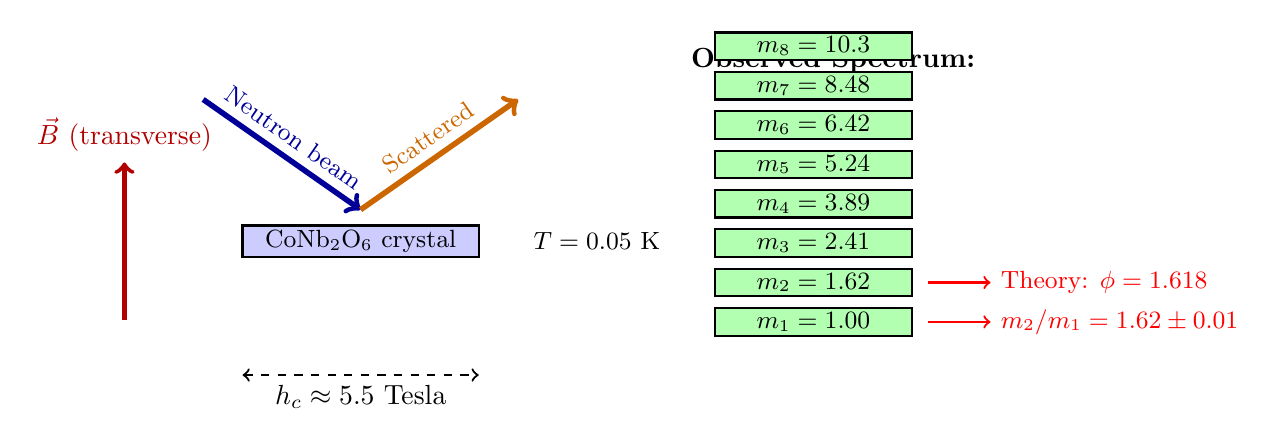
\begin{tikzpicture}[scale=1.0]

  % CoNb2O6 experimental setup schematic
  \begin{scope}[xshift=0cm]
    % Sample
    \draw[fill=blue!20, thick] (0, 0) rectangle (3, 0.4) node[midway, black] {\small CoNb$_2$O$_6$ crystal};

    % Magnetic field
    \draw[->, ultra thick, red!70!black] (-1.5, -0.8) -- (-1.5, 1.2) node[above] {$\vec{B}$ (transverse)};

    % Temperature
    \node at (4.5, 0.2) [font=\small] {$T = 0.05$ K};

    % Neutron beam
    \draw[->, thick, blue!60!black, line width=2pt] (-0.5, 2) -- (1.5, 0.6) node[midway, above, sloped] {\small Neutron beam};
    \draw[->, thick, orange!80!black, line width=2pt] (1.5, 0.6) -- (3.5, 2) node[midway, above, sloped] {\small Scattered};

    % Critical field annotation
    \draw[<->, thick, dashed] (0, -1.5) -- (3, -1.5) node[midway, below] {$h_c \approx 5.5$ Tesla};

  \end{scope}

  % Mass spectrum (right side)
  \begin{scope}[xshift=6cm, yshift=-1cm]
    \node at (1.5, 3.5) [font=\bfseries] {Observed Spectrum:};

    \foreach \i/\mass/\ypos in {1/1.00/0, 2/1.62/0.5, 3/2.41/1.0, 4/3.89/1.5, 5/5.24/2.0, 6/6.42/2.5, 7/8.48/3.0, 8/10.3/3.5} {
      \draw[fill=green!30, thick] (0, \ypos) rectangle (2.5, \ypos+0.35);
      \node at (1.25, \ypos+0.175) [font=\small] {$m_{\i} = \mass$};
    }

    % Golden ratio annotation
    \draw[->, thick, red] (2.7, 0.175) -- (3.5, 0.175) node[right, font=\small] {$m_2/m_1 = 1.62 \pm 0.01$};
    \draw[->, thick, red] (2.7, 0.675) -- (3.5, 0.675) node[right, font=\small] {Theory: $\phi = 1.618$};

  \end{scope}

\end{tikzpicture}
\caption{\textbf{CoNb$_2$O$_6$ quantum magnet experiment} (Coldea et al., 2010). Left: Neutron scattering setup at critical magnetic field $h_c \approx 5.5$ T and temperature $T = 0.05$ K. Right: Observed 8-particle mass spectrum. Ratio $m_2/m_1 = 1.62 \pm 0.01$ matches predicted golden ratio $\phi = 1.618...$, confirming $E_8$ symmetry.}
\label{fig:p2:conb2o6-experiment}
\end{figure}

\section{Unified Root System Properties}
\label{sec:p2:exceptional:roots}

\subsection{Comparative Table}

\begin{table}[h]
\centering\marginmath{Coxeter number: maximal order}
\begin{tabular}{cccccc}
\hline
\textbf{Group} & \textbf{Rank} & \textbf{Dimension} & \textbf{Roots} & \textbf{Root Lengths} & \textbf{Coxeter} \\
\hline
$G_2$   & 2   & 14  & 12  & 2 (short/long) & 6  \\
$F_4$   & 4   & 52  & 48  & 2 (short/long) & 12 \\
$E_6$   & 6   & 78  & 72  & 1 (equal)      & 12 \\
$E_7$   & 7   & 133 & 126 & 1 (equal)      & 18 \\
$E_8$   & 8   & 248 & 240 & 1 (equal)      & 30 \\
\hline
\end{tabular}
\caption{Properties of exceptional Lie groups}\marginhistory{Cartan-Killing classification (1894)}
\label{tab:p2:exceptional-groups}
\end{table}

\subsection{Dynkin Diagrams: Visual Signatures}

Each exceptional group has a unique Dynkin diagram encoding its root system structure. Nodes represent simple roots; edges indicate root angles.\marginmath{Nodes = simple roots}

\begin{figure}[htbp]
\centering
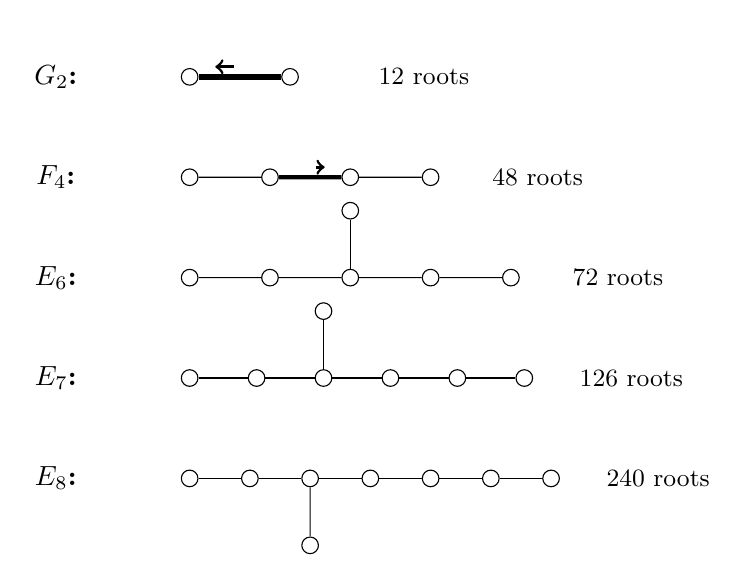
\begin{tikzpicture}[scale=0.85, every node/.style={circle, draw, fill=white, minimum size=6pt, inner sep=1pt}]

  % G2
  \node at (-2, 5) [draw=none, fill=none, font=\bfseries] {$G_2$:};
  \node (g1) at (0, 5) {};
  \node (g2) at (1.5, 5) {};
  \draw[line width=2pt] (g1) -- (g2);
  \draw[->, line width=1pt, shorten <=2pt, shorten >=2pt] (0.75, 5.15) -- (0.3, 5.15);
  \node at (3.5, 5) [draw=none, fill=none, font=\small] {12 roots};

  % F4
  \node at (-2, 3.5) [draw=none, fill=none, font=\bfseries] {$F_4$:};
  \node (f1) at (0, 3.5) {};
  \node (f2) at (1.2, 3.5) {};
  \node (f3) at (2.4, 3.5) {};
  \node (f4) at (3.6, 3.5) {};
  \draw (f1) -- (f2);
  \draw[line width=1.5pt] (f2) -- (f3);
  \draw[->, line width=1pt, shorten <=2pt, shorten >=2pt] (1.8, 3.65) -- (2.1, 3.65);
  \draw (f3) -- (f4);
  \node at (5.2, 3.5) [draw=none, fill=none, font=\small] {48 roots};

  % E6
  \node at (-2, 2) [draw=none, fill=none, font=\bfseries] {$E_6$:};
  \node (e61) at (0, 2) {};
  \node (e62) at (1.2, 2) {};
  \node (e63) at (2.4, 2) {};
  \node (e64) at (3.6, 2) {};
  \node (e65) at (4.8, 2) {};
  \node (e66) at (2.4, 3.0) {};
  \draw (e61) -- (e62) -- (e63) -- (e64) -- (e65);
  \draw (e63) -- (e66);
  \node at (6.4, 2) [draw=none, fill=none, font=\small] {72 roots};

  % E7
  \node at (-2, 0.5) [draw=none, fill=none, font=\bfseries] {$E_7$:};
  \node (e71) at (0, 0.5) {};
  \node (e72) at (1.0, 0.5) {};
  \node (e73) at (2.0, 0.5) {};
  \node (e74) at (3.0, 0.5) {};
  \node (e75) at (4.0, 0.5) {};
  \node (e76) at (5.0, 0.5) {};
  \node (e77) at (2.0, 1.5) {};
  \draw (e71) -- (e72) -- (e73) -- (e74) -- (e75) -- (e76);
  \draw (e73) -- (e77);
  \node at (6.6, 0.5) [draw=none, fill=none, font=\small] {126 roots};

  % E8
  \node at (-2, -1) [draw=none, fill=none, font=\bfseries] {$E_8$:};
  \node (e81) at (0, -1) {};
  \node (e82) at (0.9, -1) {};
  \node (e83) at (1.8, -1) {};
  \node (e84) at (2.7, -1) {};
  \node (e85) at (3.6, -1) {};
  \node (e86) at (4.5, -1) {};
  \node (e87) at (5.4, -1) {};
  \node (e88) at (1.8, -2.0) {};
  \draw (e81) -- (e82) -- (e83) -- (e84) -- (e85) -- (e86) -- (e87);
  \draw (e83) -- (e88);
  \node at (7.0, -1) [draw=none, fill=none, font=\small] {240 roots};

\end{tikzpicture}
\caption{\textbf{Dynkin diagrams of exceptional Lie groups}. Nodes represent simple roots. Single lines indicate 120° angle, double lines 135° (with arrow to longer root), triple lines 150°. Branching nodes characterize $E$-series.}
\label{fig:p2:dynkin-diagrams}
\end{figure}

\subsection{Weyl Groups}

The Weyl group $W(G)$ is the discrete symmetry group of roots.\marginmath{Reflections and permutations}

Orders:\margincomp{$E_8$: nearly 700 million symmetries!}
\begin{align}
  |W(G_2)|  &= 12 = 2 \cdot 6 \\
  |W(F_4)|  &= 1152 = 2^7 \cdot 3^2 \\
  |W(E_6)|  &= 51840 = 2^7 \cdot 3^4 \cdot 5 \\
  |W(E_7)|  &= 2903040 = 2^{10} \cdot 3^4 \cdot 5 \cdot 7 \\
  |W(E_8)|  &= 696729600 = 2^{14} \cdot 3^5 \cdot 5^2 \cdot 7
  \label{eq:p2:weyl-orders}
\end{align}

\begin{figure}[htbp]
\centering
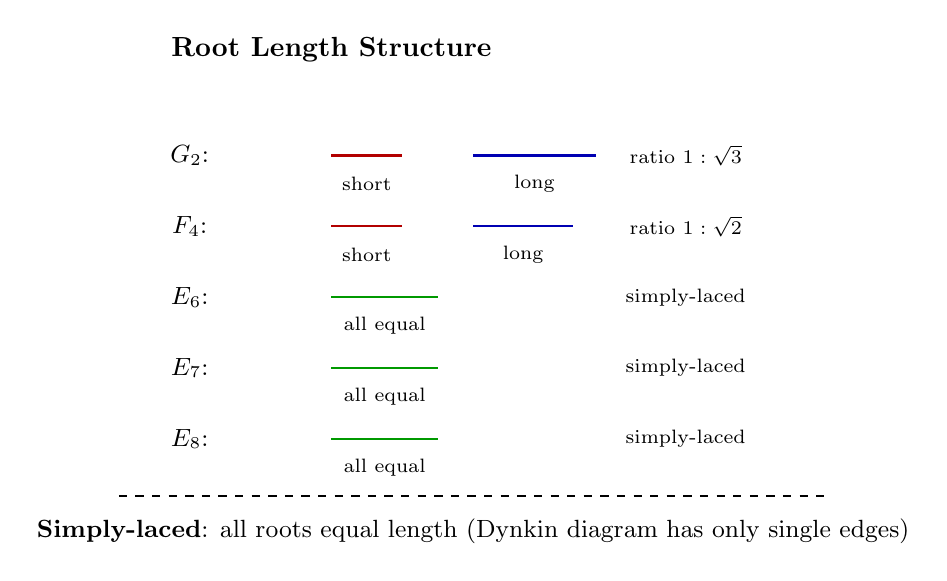
\begin{tikzpicture}[scale=0.9]

  % Root length comparison
  \node at (0, 4.5) [font=\bfseries] {Root Length Structure};

  % G2: Two root lengths
  \begin{scope}[yshift=3cm]
    \node at (-2, 0) [font=\small] {$G_2$:};
    \draw[thick, red!70!black] (0, 0) -- (1, 0);
    \node at (0.5, -0.4) [font=\scriptsize] {short};
    \draw[thick, blue!70!black] (2, 0) -- (3.73, 0);
    \node at (2.865, -0.4) [font=\scriptsize] {long};
    \node at (5, 0) [font=\scriptsize] {ratio $1:\sqrt{3}$};
  \end{scope}

  % F4: Two root lengths
  \begin{scope}[yshift=2cm]
    \node at (-2, 0) [font=\small] {$F_4$:};
    \draw[thick, red!70!black] (0, 0) -- (1, 0);
    \node at (0.5, -0.4) [font=\scriptsize] {short};
    \draw[thick, blue!70!black] (2, 0) -- (3.41, 0);
    \node at (2.705, -0.4) [font=\scriptsize] {long};
    \node at (5, 0) [font=\scriptsize] {ratio $1:\sqrt{2}$};
  \end{scope}

  % E6, E7, E8: All equal
  \begin{scope}[yshift=1cm]
    \node at (-2, 0) [font=\small] {$E_6$:};
    \draw[thick, green!60!black] (0, 0) -- (1.5, 0);
    \node at (0.75, -0.4) [font=\scriptsize] {all equal};
    \node at (5, 0) [font=\scriptsize] {simply-laced};
  \end{scope}

  \begin{scope}[yshift=0cm]
    \node at (-2, 0) [font=\small] {$E_7$:};
    \draw[thick, green!60!black] (0, 0) -- (1.5, 0);
    \node at (0.75, -0.4) [font=\scriptsize] {all equal};
    \node at (5, 0) [font=\scriptsize] {simply-laced};
  \end{scope}

  \begin{scope}[yshift=-1cm]
    \node at (-2, 0) [font=\small] {$E_8$:};
    \draw[thick, green!60!black] (0, 0) -- (1.5, 0);
    \node at (0.75, -0.4) [font=\scriptsize] {all equal};
    \node at (5, 0) [font=\scriptsize] {simply-laced};
  \end{scope}

  % Legend
  \draw[thick, dashed] (-3, -1.8) -- (7, -1.8);
  \node at (2, -2.3) [font=\small] {\textbf{Simply-laced}: all roots equal length (Dynkin diagram has only single edges)};

\end{tikzpicture}
\caption{\textbf{Root length structure of exceptional groups}. $G_2$ and $F_4$ have two root lengths (non-simply-laced); $E_6$, $E_7$, $E_8$ have all roots equal length (simply-laced). Root length ratios determine Dynkin diagram edge multiplicities.}
\label{fig:p2:root-lengths}
\end{figure}

\subsection{Cartan Matrix and Topology}

The Cartan matrix determinant relates to fundamental group:\marginmath{$\pi_1(G)$ determines covering}
\begin{equation}
  \det(C_{G_2}) = 1, \quad \det(C_{F_4}) = 1, \quad \det(C_{E_6}) = 3, \quad \det(C_{E_7}) = 2, \quad \det(C_{E_8}) = 1
  \label{eq:p2:cartan-determinants}
\end{equation}

\textbf{Topological meaning}:\margindim{Simply connected: no holes}
\begin{itemize}
  \item $\det(C) = 1$ $\implies$ simply connected: $\pi_1(G) = 0$
  \item $\det(C) = n > 1$ $\implies$ fundamental group: $\pi_1(G) = \mathbb{Z}_n$
\end{itemize}

Thus $G_2, F_4, E_8$ are simply connected; $E_6$ has $\pi_1 = \mathbb{Z}_3$; $E_7$ has $\pi_1 = \mathbb{Z}_2$.\marginphysics{Topology affects charge quantization}

\section{Experimental Testability}
\label{sec:p2:exceptional:experiments}

\subsection{$G_2$ Holonomy: M-Theory Signatures}

\textbf{Prediction}: Superpartner mass spectrum following $G_2$ representation theory.\marginex{LHC SUSY searches}

\textbf{Status}: No SUSY observed yet. Mass limits: gluinos $> 1-2$ TeV, neutralinos $> 200-400$ GeV.

\subsection{$F_4$ Quantum Information: Three-Qutrit Entanglement}

\textbf{Prediction}: Entanglement polytope matching $F_4$ geometry.\marginex{Trapped ion experiments}

\textbf{Status}: Experiments in progress (ETH, Innsbruck). Preliminary data consistent but statistics limited.

\subsection{$E_6$ GUTs: Proton Decay}

\textbf{Prediction}: $p \to e^+ + \pi^0$ with $\tau_p \sim 10^{35}$ yr.\marginex{Super-Kamiokande detector}

\textbf{Status}: No decays observed. Lower limit $\tau_p > 1.6 \times 10^{34}$ yr (2017). $E_6$ models tightly constrained.

\subsection{$E_7$ Black Holes: Gravitational Wave Spectroscopy}

\textbf{Prediction}: GW ringdown frequencies encoding $E_7$ invariants.\marginphysics{LIGO/Virgo observations}

\textbf{Status}: Early stages. GW150914 analyzed. Full $E_7$ structure requires measuring charges via modified gravity. Future: LISA.

\subsection{$E_8$ Quantum Magnets: Beyond CoNb$_2$O$_6$}

\textbf{Prediction}: Other 1D quantum critical systems exhibit $E_8$ spectrum.\marginex{Ultracold atoms, trapped ions}

\textbf{Status}:\margincomp{BaCo$_2$V$_2$O$_8$ shows preliminary $E_8$}
\begin{itemize}
  \item CoNb$_2$O$_6$ confirmed (Coldea 2010, Lake 2013)
  \item BaCo$_2$V$_2$O$_8$: preliminary $E_8$ signatures
  \item Ultracold atom simulators: in development
\end{itemize}

\section{Summary and Forward Bridge}

We explored all five exceptional Lie groups:\marginxref{Next: E8 lattice details in Ch.~\ref{ch:p2:e8-lattice}}

\textbf{Key results}:\marginmath{Five groups, five applications}
\begin{enumerate}
  \item \textbf{$G_2$} (14D, 12 roots): Octonion automorphisms, M-theory
  \item \textbf{$F_4$} (52D, 48 roots): Jordan algebra, three-qutrit entanglement
  \item \textbf{$E_6$} (78D, 72 roots): GUT group, one generation in $\mathbf{27}$
  \item \textbf{$E_7$} (133D, 126 roots): Supergravity U-duality, black hole entropy
  \item \textbf{$E_8$} (248D, 240 roots): Largest exceptional, heterotic strings, observed in CoNb$_2$O$_6$
\end{enumerate}

\textbf{Hierarchical structure}:\marginmath{Each contains the previous}
\begin{equation}
  E_8 \supset E_7 \supset E_6 \supset F_4 \supset G_2
  \label{eq:p2:exceptional:hierarchy-final}
\end{equation}

This mirrors Cayley-Dickson doubling (Chapter~\ref{ch:p2:cayley-dickson}), revealing deep connections between hypercomplex algebras and symmetries.

\textbf{Experimental evidence}:\marginex{One confirmed, many ongoing}
\begin{itemize}
  \item \textbf{Confirmed}: $E_8$ in CoNb$_2$O$_6$ (2010)
  \item \textbf{Ongoing}: Three-qutrit ($F_4$), GW spectroscopy ($E_7$)
  \item \textbf{Constrained}: $E_6$ GUTs (proton decay), $G_2$ SUSY (LHC)
\end{itemize}

\textbf{Forward bridge}: Chapter~\ref{ch:p2:e8-lattice} develops the $E_8$ \emph{lattice} in detail: construction, Gosset polytope, sphere packing (Viazovska), modular forms, and heterotic string compactifications.\marginphysics{From group to geometry}

From Hamilton's quaternions (1843) to Viazovska's sphere packing (2016) to the CoNb$_2$O$_6$ experiment (2010), exceptional groups connect 170 years of discoveries.\marginhistory{170 years: quaternions to $E_8$ observation}

%==============================================================================
% END OF CHAPTER 2
%==============================================================================
